%--------------------------------------------CAPA FISICA ------------------------------------------------------%

 
\subsection{Capa física}
Los elementos físicos son una extensión de la capa tecnológica para modelar el mundo físico. Solo incluyen elementos estructurales, activos y pasivos; no se definen elementos de comportamiento físico específicos. Los elementos de tecnología física se pueden combinar con otros elementos tecnológicos (como un dispositivo) y ser parte del mismo nodo, para modelar una pieza integrada de tecnología operativa y de información.

Las interrelaciones de elementos físicos están formadas principalmente por la infraestructura logística. El elemento de ruta de la capa de tecnología modela la relación entre dos o más nodos, a través de los cuales estos nodos pueden intercambiar información o material. La realización física de un camino se modela con una red de distribución; es decir, una conexión física entre dos o más equipos (u otras redes físicas). Esto se puede utilizar para modelar, por ejemplo, redes ferroviarias o de carreteras, el suministro de agua, la red eléctrica o la red de gas.

La Tabla \ref{tab:Tabla de la capa física} ofrece una descripción general de los elementos de la capa tecnológica, con sus definiciones.\cite{archimate} 


\begin{longtable}{|p{0.15\linewidth}|p{0.45\linewidth}|p{0.4\linewidth} |}
    \caption{Tabla de la capa física}
    \\
    \hline
    \rowcolor[HTML]{AFC5F6} 
    \textbf{Elemento} & \textbf{Descripción} & \textbf{Notación} \\
    \hline
    \endhead
    \hline
    \multicolumn{3}{r}{\textit{Continúa en la siguiente página}} \\
    \endfoot
    \hline
    \endlastfoot
    \label{tab:Tabla de la capa física}
    %Contenido 1 &
    %\lipsum[1] &
    %Datos A1
    %& Datos B1
    %\\
    %\hline



    Equipo
    &
    Representa una o más máquinas, herramientas 
    o instrumentos físicos que pueden crear, utilizar, 
    almacenar, mover o transformar materiales.
    &
\begin{center}
    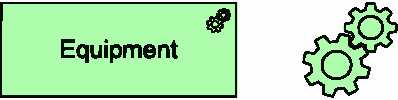
\includegraphics[width=0.8\linewidth]{imgs/capa_fisica/Equipment.pdf}
\end{center} 
    \\ \hline



    Instalación
    &
    Representa una estructura física o entorno.
    &
\begin{center}
    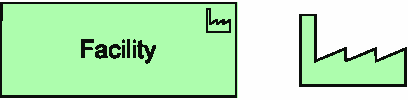
\includegraphics[width=0.8\linewidth]{imgs/capa_fisica/Facility.pdf}
\end{center} 
    \\ \hline



    Red de distribución
    &
    Representa una red física utilizada para 
    transportar materiales o energía.
    &
\begin{center}
    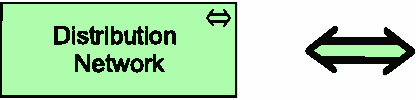
\includegraphics[width=0.8\linewidth]{imgs/capa_fisica/Distribution network.pdf}
\end{center} 
    \\ \hline



    Material
    &
    Representa materia física tangible o energía.
    &
\begin{center}
    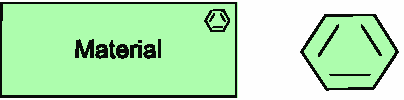
\includegraphics[width=0.8\linewidth]{imgs/capa_fisica/Material.pdf}
\end{center} 
    \\ \hline


\end{longtable}